\RequirePackage[l2tabu, orthodox]{nag}
\documentclass{article}
\usepackage{mathptmx}
\usepackage[T1]{fontenc}
\usepackage[latin9]{inputenc}
\usepackage{microtype}
\usepackage{calc}
\usepackage{siunitx}
\usepackage{amsmath}
\usepackage{amssymb}
\usepackage{graphicx}
\usepackage{subdepth}
\usepackage{cite}
\usepackage{url}
\usepackage{notoccite}
%\usepackage{nag}
\usepackage[letterpaper]{geometry}
\usepackage{hyperref}
\usepackage{cleveref}
\crefname{equation}{equation}{equations}
\title{Newtonian approximation in Causal Dynamical Triangulations}
\author{Adam Getchell}
\date{\today}
\begin{document}
\maketitle
\tableofcontents

\section{Newton's Law of Gravitation from General Relativity}

\subsection{Vacuum solution to the Weyl metric}

Starting from the most general cylindrically symmetric (Weyl) metric \cite{synge_relativity}:

\begin{equation}
ds^{2}=e^{2\lambda}dt^{2}-e^{2\left(\nu-\lambda\right)}\left(dr^{2}+dz^{2}\right)-r^{2}e^{-2\lambda}d\phi^{2}\label{eq:weyl-metric}
\end{equation}

\begin{equation}
g_{\mu\nu}=\left(\begin{array}{cccc}
e^{2\lambda}dt^{2} & 0 & 0 & 0\\
0 & -e^{2\left(\nu-\lambda\right)}dr^{2} & 0 & 0\\
0 & 0 & -e^{2\left(\nu-\lambda\right)}dz^{2} & 0\\
0 & 0 & 0 & -\frac{r^{2}}{e^{2\lambda}}d\phi^{2}
\end{array}\right)\label{eq:general-axisymmetric-static-matrix-metric}
\end{equation}

In this coordinate basis, the definition of the Christoffel connection is: \cite{carroll2003spacetime} 
\begin{equation}
\Gamma_{\mu\nu}^{\lambda}=\frac{1}{2}g^{\lambda\sigma}\left(\partial_{\mu}g_{\nu\sigma}+\partial_{\nu}g_{\sigma\mu}-\partial_{\sigma}g_{\mu\nu}\right)
\end{equation}

The non-zero Christoffel connections are:
\begin{equation}
\begin{aligned}
\Gamma^{t}_{tr}&=\partial_{r}\lambda\\
\Gamma^{t}_{tz}&=\partial_{z}\lambda\\
\Gamma^{r}_{tt}&=e^{4\lambda-2\nu}\partial_{r}\lambda\\
\Gamma^{r}_{rr}&=\partial_{r}\nu-\partial_{r}\lambda\\
\Gamma^{r}_{rz}&=\partial_{z}\nu-\partial_{z}\lambda\\
\Gamma^{r}_{zz}&=\partial_{z}\lambda-\partial_{z}\nu\\
\Gamma^{r}_{\phi\phi}&=re^{-2\nu}\left(r\partial_{r}\lambda-1\right)\\
\Gamma^{z}_{tt}&=e^{4\lambda-2\nu}\partial_{z}\lambda\\
\Gamma^{z}_{rr}&=\partial_{z}\lambda-\partial_{z}\nu\\
\Gamma^{z}_{rz}&=\partial_{r}\nu-\partial_{r}\lambda\\ 
\Gamma^{z}_{zz}&=\partial_{r}\nu-\partial_{r}\lambda\\
\Gamma^{z}_{\phi\phi}&=r^{2}e^{-2\nu}\partial_{z}\lambda\\
\Gamma^{\phi}_{r\phi}&=\frac{1}{r}-\partial_{r}\lambda\\
\Gamma^{\phi}_{z\phi}&=-\partial_{z}\lambda\\
\end{aligned}
\label{eq:christoffel-connections}
\end{equation}

The components of the Riemann tensor are given by:
\begin{equation}
R_{\sigma\mu\nu}^{\rho}=\partial_{\mu}\Gamma_{\nu\sigma}^{\rho}-\partial_{\nu}\Gamma_{\mu\sigma}^{\rho}+\Gamma_{\mu\lambda}^{\rho}\Gamma_{\nu\sigma}^{\lambda}-\Gamma_{\nu\lambda}^{\rho}\Gamma_{\mu\sigma}^{\lambda}
\end{equation}

Using the properties of the Riemann tensor:
\begin{equation}
\begin{aligned}
R_{\rho\sigma\mu\nu}&=-R_{\rho\sigma\nu\mu}\\
R_{\rho\sigma\mu\nu}&=-R_{\sigma\rho\mu\nu}\\
R_{\rho\sigma\mu\nu}&=R_{\mu\nu\rho\sigma}\\
R_{\rho[\sigma\mu\nu]}&=0\\
\end{aligned}
\end{equation}
The non-zero components of the Riemann tensor are:
\begin{equation}
\begin{aligned}
R^{t}_{rtr}&=-\partial^{2}_{r}\lambda+\left(\partial_{z}\lambda\right)^{2}-2\left(\partial_{r}\lambda\right)^{2}+\partial_{r}\lambda\partial_{r}\nu-\partial_{z}\lambda\partial_{z}\nu\\
R^{t}_{rtz}&=-\partial_{r}\partial_{z}\lambda-3\partial_{r}\lambda\partial_{z}\lambda+\partial_{r}\lambda\partial_{z}\nu+\partial_{r}\nu\partial_{z}\lambda\\
R^{t}_{ztz}&=-\partial^{2}_{z}\lambda-2\left(\partial_{z}\lambda\right)^{2}+\left(\partial_{r}\lambda\right)^{2}-\partial_{r}\lambda\partial_{r}\nu+\partial_{z}\lambda\partial_{z}\nu\\
R^{t}_{\phi t\phi}&=re^{-2\nu}\left(r\left(\partial_{r}\lambda\right)^{2}-\partial_{r}\lambda+r\left(\partial_{z}\lambda\right)^{2}\right)\\
R^{r}_{zrz}&=\partial^{2}_{r}\lambda-\partial^{2}_{r}\nu+\partial^{2}_{z}\lambda-\partial^{2}_{z}\nu\\
R^{z}_{\phi z\phi}&=re^{-2\nu}\left(r\partial^{2}_{z}\lambda-r\partial_{z}\lambda\partial_{z}\nu+r\partial_{r}\lambda\partial_{r}\nu-r\left(\partial_{r}\lambda\right)^{2}+\partial_{r}\lambda-\partial_{r}\nu\right)\\
R^{z}_{\phi\phi r}&=re^{-2\nu}\left(-r\partial_{r}\partial_{z}\lambda+r\partial_{r}\nu\partial_{z}\lambda-r\partial_{r}\lambda\partial_{z}\lambda+r\partial_{r}\lambda\partial_{z}\nu-\partial_{z}\nu\right)\\
R^{\phi}_{r\phi r}&=\partial^{2}_{r}\lambda+\frac{1}{r}\partial_{r}\nu-\partial_{r}\lambda\partial_{r}\nu-\left(\partial_{z}\lambda\right)^{2}+\partial_{z}\lambda\partial_{z}\nu+\frac{1}{r}\partial_{r}\lambda\\
\end{aligned}
\end{equation}

The Ricci tensor is given by:
\begin{equation}
R_{\mu\nu}=R_{\mu\lambda\nu}^{\lambda}
\end{equation}

The non-zero components of the Ricci tensor are:
\begin{equation}
\begin{aligned}
R_{tt}&=\frac{e^{4\lambda-2\nu}}{r}\left(r\partial^{2}_{r}\lambda+r\partial^{2}_{z}\lambda+\partial_{r}\lambda\right)\\
R_{rr}&=\partial^{2}_{r}\lambda-\partial^{2}_{r}\nu+\partial^{2}_{z}\lambda-\partial^{2}_{z}\nu-2\left(\partial_{r}\lambda\right)^{2}+\frac{1}{r}\partial_{r}\lambda+\frac{1}{r}\partial_{r}\nu\\
R_{rz}&=\frac{1}{r}\partial_{z}\nu-2\partial_{r}\lambda\partial_{z}\lambda\\
R_{zz}&=\partial^{2}_{r}\lambda-\partial^{2}_{r}\nu+\partial^{2}_{z}\lambda-\partial^{2}_{z}\nu-2\left(\partial_{z}\lambda\right)^{2}+\frac{1}{r}\partial_{r}\lambda-\frac{1}{r}\partial_{r}\nu\\
R_{\phi\phi}&=re^{-2\nu}\left(r\partial^{2}_{r}\lambda+r\partial^{2}_{z}\lambda+\partial_{r}\lambda\right)
\end{aligned}
\label{eq:ricci-tensor-components}
\end{equation}

Einstein's equation in a vacuum is:
\begin{equation}
R_{\mu\nu}=0\label{eq:vacuum-solutions}
\end{equation}

Applying this complete set of relations to \Cref{eq:ricci-tensor-components} gives the following:
\begin{equation}
\partial^{2}_{r}\lambda+\frac{1}{r}\partial_{r}\lambda+\partial^{2}_{z}\lambda=0\label{eq:laplace}
\end{equation}
\begin{equation}
\partial_{r}\nu=r\left(\partial^{2}_{r}\nu+\partial^{2}_{z}\nu+2\left(\partial_{r}\lambda\right)^{2}\right)\label{eq:R_rr=0}
\end{equation}
\begin{equation}
\partial_{z}\nu=2r\partial_{r}\lambda\partial_{z}\lambda\label{eq:nu_z}
\end{equation}
\begin{equation}
\partial^{2}_{r}\nu+\partial^{2}_{z}\nu+\left(\partial_{r}\lambda\right)^{2}+\left(\partial_{z}\lambda\right)^{2}=0\label{eq:R_phiphi=0}
\end{equation}

\Cref{eq:laplace} is the two-dimensional Laplace equation in cylindrical coordinates. Plugging \Cref{eq:R_phiphi=0} into \Cref{eq:R_rr=0} gives:

\begin{equation}
\partial_{r}\nu=r\left(\left(\partial_{r}\lambda\right)^{2}-\left(\partial_{z}\lambda\right)^{2}\right)\label{eq:nu_r}
\end{equation}

Using \Cref{eq:nu_z,eq:nu_r} we find solutions for $\nu$ are given by:
\begin{equation}
\nu=\int r[\left(\left(\partial_{r}\lambda\right)^{2}-\left(\partial_{z}\lambda\right)^{2}\right)dr+\left(2\partial_{r}\lambda\partial_{z}\lambda\right)dz]\label{eq:nu}
\end{equation}

\subsection{Elementary Flatness}

In order to be certain that our spacetime is truly flat, we will
impose the condition of elementary flatness: the ratio of the
circumference and radius is equal to $2\pi$. This will give us restrictions on our solutions for $\lambda\left(r,z\right)$ and $\nu\left(r,z\right)$.

To do this we will first integrate in the $\hat{\phi}$ direction at
some $r$ and then divide by $r$. Doing this gives:

\begin{equation}
  \label{eq:phi-hat-length}
  L=\int ds =
  \int_0^{2\pi}\sqrt{-r^2e^{-2\lambda}d\phi^2}=\pm\frac{2\pi r}{e^{\lambda}}
\end{equation}

Then the condition that $\frac{L}{r}=2\pi$ holds provided that
$e^{-\lambda}=1$. That is, $\lambda(0,z)\rightarrow 0$. But since
$\frac{L}{r}$ is not well-defined as $r\rightarrow 0$, this is a sign
that we need to look more carefully at the $z$-axis.

Next, we will parallel transport a vector $V$ about the $z$-axis in
the $\hat{\phi}$ direction and demand that the values
for $\phi=0$ and $\phi=2\pi$ are equal. 

The equation for parallel transport is generally given by:
  	
\begin{equation}
\begin{array}{rcl} \frac{D}{d\lambda}=\frac{dx^{\mu}}{d\lambda}\nabla_{\mu}=0 & \mbox{along} & x^{\mu}\left(\lambda\right)	  	
\end{array}
\end{equation}	  	
That is, the directional covariant derivative is equal to zero along
the curve $x^{\mu}$ parameterized by $\lambda$. For a vector this can
be simply written as:

\begin{equation}
\label{eq:x-par-xport}
\nabla_\mu V^{\nu}=\partial_\mu V^\nu+\Gamma^\nu_{\mu\lambda} V^\lambda=0
\end{equation}	  	
Starting with parallel transport along $\hat{e}_{\phi}$, \Cref{eq:x-par-xport} along with the relevant Christoffel symbols $\Gamma^{r}_{\phi\phi}$, $\Gamma^{z}_{\phi\phi}$, $\Gamma^{\phi}_{\phi r}$, and $\Gamma^{\phi}_{\phi z}$ gives:
	  	
\begin{equation}
\begin{aligned}
\partial_{\phi}V^{r}+\Gamma^{r}_{\phi\phi}V^{\phi}&=0\\
\partial_{\phi}V^{z}+\Gamma^{z}_{\phi\phi}V^{\phi}&=0\\
\partial_{\phi}V^{\phi}+\Gamma^{\phi}_{\phi r}V^{r}+\Gamma^{\phi}_{\phi z}V^{z}&=0\\
\end{aligned}
\end{equation}
Plugging in the values from \Cref{eq:christoffel-connections}, our equations are: 

\begin{equation}
\partial_{\phi}V^{r}+\left(re^{-2\nu}\left(r\partial_{r}\lambda-1\right)\right)V^{\phi}=0\label{eq:V-r-phi}
\end{equation}

\begin{equation}
\label{eq:V_z-V_phi}
\partial_{\phi}V^{z}+\left(r^{2}e^{-2\nu}\partial_{z}\lambda\right)V^{\phi}=0
\end{equation}

\begin{equation}
\partial_{\phi}V^{\phi}+\left(\frac{1}{r}-\partial_{r}\lambda\right)V^{r}-\partial_{z}\lambda V^{z}=0\label{eq:V-phi-r-z}
\end{equation}

Differentiating \Cref{eq:V-phi-r-z} with respect to $\phi$ and plugging it into \Cref{eq:V-r-phi} gives:

\begin{equation}
\partial^{2}_{\phi}V^{\phi}-\partial_z\lambda\partial_{\phi}V^z+r^{2}e^{-2\nu}\left(\partial_r\lambda-\frac{1}{r}\right)^2V^{\phi}=0
\end{equation}
Plugging in the expression for $\partial_{\phi}V^z$ from
\Cref{eq:V_z-V_phi} and letting 

\begin{equation}
\label{eq:def-chi}
\chi=re^{-\nu}(\partial_r\lambda+\partial_z\lambda-\frac{1}{r})
\end{equation}
We have the simple differential equation:

\begin{equation}
\partial^2_\phi V^\phi+\chi^2 V^\phi=0
\end{equation}
For which the solution is:

\begin{equation}
V^{\phi}=A\sin\chi\phi+B\cos\chi\phi
\end{equation}
Therefore, integrating \Cref{eq:V-r-phi} with respect to $\phi$ we get:

\begin{equation}
V^{r}=\frac{re^{-\nu}(\partial_r\lambda-\frac{1}{r})}{\partial_r\lambda+\partial_z\lambda-\frac{1}{r}}\left(A\cos\chi\phi-B\sin\chi\phi\right)
\end{equation}

And from \Cref{eq:V-phi-r-z}:

\begin{equation}
V^{z}=\frac{\partial_z\lambda e^{-\nu}}{\partial_r\lambda+\partial_{z}\lambda-\frac{1}{r}}\left(A\cos\chi\phi-B\sin\chi\phi\right)
\end{equation}

At $\phi=0$ we have $V^\phi=1$ and $V^r=r_0$ (leaving aside for the
moment $V^z$, since we are free to parallel transport about $\phi$
anywhere along the z-axis). Then the condition that $V^\phi=1$ leads to
$B=1$. Likewise, setting $V^r=r_0$ leads to:

\begin{equation}
  \label{eq:conditions}
  \frac{Ar_0 e^{-\nu}(\partial_r\lambda-\frac{1}{r_0})}{\partial_r\lambda+\partial_z\lambda-\frac{1}{r_0}}=r_0
\end{equation}

We set $A=1$ for convenience. Then from \Cref{eq:conditions}, provided
that $\frac{1}{r_0}\gg\partial_r\lambda+\partial_z\lambda$ for small
$r_0$ one finds that $e^{-\nu}\rightarrow 1$, or $\nu(r_0,z)\rightarrow
0$. As $r_0$ is completely arbitrary so we can characterize this as:

\begin{equation}
  \label{eq:nu-elem-flat}
  \lim_{r\rightarrow 0}\nu=0
\end{equation}

The general expression for the vector is then:

\begin{equation}
\label{eq:v-from-par-transport}
V=\left(\cos\chi\phi-\sin\chi\phi\right)\left(\frac{re^{-\nu}(\partial_r\lambda-\frac{1}{r})}{\partial_r\lambda+\partial_z\lambda-\frac{1}{r}}\hat{e}_{r}+\frac{\partial_z\lambda e^{-\nu}}{\partial_r\lambda+\partial_{z}\lambda-\frac{1}{r}}\hat{e}_{z}\right)+\left(\sin(\chi\phi)+\cos(\chi\phi)\right)\hat{e}_{\phi}
\end{equation}

Thus, the requirement that the vector is identical at $\phi=2\pi$
after being transported around the circle starting at $\phi=0$ at an arbitrary
distance $r_0$ is:

\begin{equation}
  \label{eq:v-par-transport-2pi}
  V=r_0 e^{-\nu}\left(\cos(2\pi\chi)-\sin(2\pi\chi)\right)\left(\hat{e}_{r}\mp\hat{e}_{z}\right)+\left(\sin(2\pi\chi+\cos(2\pi\chi)\right)\hat{e}_{\phi}
\end{equation}


\subsection{Matter solution to the Weyl metric}

In principle, we have solutions for axially symmetric static vacuum spacetimes. We now wish to add matter. If the object is also axially symmetric and static, then we can consider solutions in the form of an external metric $\emph{E}$ and an internal metric $\emph{I}$, where $\emph{E}$ is given by \Cref{eq:weyl-metric,eq:nu}.

The solution of Laplace's equation for a point particle of mass $\mu$ at
$z=z_{0}$ is well known \cite{letelier1997superposition}:

\begin{equation}
\lambda (r,z)=-\frac{\mu}{\sqrt{r^{2}+\left(z-z_{0}\right)^{2}}}\label{eq:1-m}
\end{equation}

Likewise, we can easily verify for a single particle that the solution
for $\nu$ from \Cref{eq:nu,eq:1-m} is (setting integration constants equal to zero):
\begin{equation}
\nu (r,z)=-\frac{\mu^{2}r^{2}}{\left(r^{2}+\left(z-z_{0}\right)^{2}\right)^{2}}
\end{equation}

Consider \Cref{fig:single-mass}, consisting of a single cylindrically symmetric mass.

\begin{figure}
\centering
\caption[A single cylindrically symmetric mass]
{A single cylindrically symmetric mass, adapted from \cite{synge_relativity} Fig. 10.1}
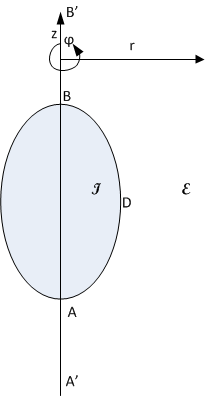
\includegraphics[width=40mm]{Figure1.png}
\label{fig:single-mass}
\end{figure}

Equation \eqref{eq:nu} includes a constant, which we can set by choosing that $\nu=0$ at \emph{A}. So, $\nu=0$ along the z-axis from \emph{A'} to \emph{A}. The same applies from \emph{B} to \emph{B'}. Then our path \emph{ADB} may be deformed into an infinite semicircle.



\begin{figure}
\centering
\caption[Two cylindrically symmetric masses]
{Two cylindrically symmetric masses, adapted from \cite{synge_relativity} Figure 10.2}
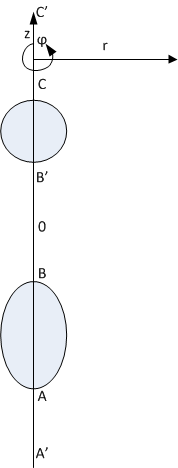
\includegraphics[width=40mm]{Figure2.png}
\label{fig:two-masses}
\end{figure}


Now consider two bodies, as in Figure \ref{fig:two-masses}. Since solutions to Laplace's equation are linear, we have:

\begin{equation}
\lambda (r,z)=-\frac{\mu_{1}}{R_{1}}-\frac{\mu_{2}}{R_{2}}\label{eq:2-m}
\end{equation}

Plugging this into Equation \eqref{eq:nu} yields:

\begin{equation}
\nu (r,z)=-\frac{\mu_{1}^{2}r^{2}}{R_{1}^{4}}-\frac{\mu_{2}^{2}r^{2}}{R_{2}^{4}}+\frac{4\mu_{1}\mu_{2}}{\left(z_{1}-z_{2}\right)^{2}}\frac{r^{2}+\left(z-z_{1}\right)\left(z-z_{2}\right)}{R_{1}R_{2}}
\end{equation}

\begin{equation}
R_{i}=\sqrt{r^{2}+\left(z-z_{i}\right)^{2}}
\end{equation}

In this case, we expect $\nu=0$ along \emph{A'A} and \emph{C'C} as before. But there is no $\emph{a priori}$ reason to think that $\nu=0$ along \emph{B'B}.
This means that our vacuum solution fails along the z-axis. Therefore, there must be a strut of matter, i.e. a metric \emph{I} such that $R_{\mu\nu}\neq 0$, along the z-axis \emph{B'B} separating the two objects. This corresponds with the expectation that two masses will attract each other and not remain at rest.

Indeed, if we apply the condition that $r=0$ we get:

\begin{equation}
\nu (0,z)=\frac{4\mu_{1}\mu_{2}}{\left(z_{1}-z_{2}\right)^{2}}\label{eq:nu_r=0}
\end{equation}

Which means that in order for Equation \eqref{eq:elem-flat} to hold, our strut must have:

\begin{equation}
\nu=-\frac{4\mu_{1}\mu_{2}}{\left(z_{1}-z_{2}\right)^{2}}
\end{equation}

To get the force on the strut, we can integrate the z-component of the stress-energy tensor over the area:

\begin{equation}
F_{z}=\int T_{zz}d\sigma
\end{equation}

We can get the stress-energy tensor from Einstein's equation:

\begin{equation}
G_{\mu\nu}\equiv R_{\mu\nu}-\frac{1}{2}Rg_{\mu\nu}=8\pi GT_{\mu\nu}\label{eq:einstein}
\end{equation}

We have all of the relevant components, except the Ricci scalar:

\begin{equation}
R=R_{\mu}^{\mu}=g^{\mu\nu}R_{\mu\nu}
\end{equation}

Which is:

\begin{equation}
R=2e^{2\left(\lambda-\nu\right)}\left(\partial^{2}_{r}\nu+\partial^{2}_{z}\nu-\partial^{2}_{r}\lambda-\partial^{2}_{z}\lambda+\left(\partial_{r}\lambda\right)^{2}+\left(\partial_{z}\lambda\right)^{2}-\frac{1}{r}\partial_{r}\lambda\right)\label{eq:R}
\end{equation}

Recall that earlier we asserted in Equation \eqref{eq:vacuum-solutions} that we had a vacuum solution. In order for this to be true, our Ricci scalar better be equal to zero, since a vacuum solution actually corresponds to:

\begin{equation}
G_{\mu\nu}=0
\end{equation}

Using Equations \eqref{eq:laplace} and \eqref{eq:R_phiphi=0} and plugging them into Equation (\ref{eq:R}) we see that this is indeed the case.

Continuing, we get:

\begin{equation}
G_{zz}=\left(\partial_{r}\lambda\right)^{2}-\left(\partial_{z}\lambda\right)^{2}-\frac{1}{r}\partial_{r}\nu \label{eq:G_zz}
\end{equation}

Again, generally speaking $G_{zz}=0$, which we can see by plugging Equation (\ref{eq:nu_r}) into Equation \eqref{eq:G_zz}. So we have this object which is zero everywhere except along the z-axis.

That object is a conical singularity \cite{araujo_static_1995}.

We can solve this problem by using the Gauss-Bonnet theorem: \cite{weisstein_gauss-bonnet}

\begin{equation}
\iint_{M} KdA=2\pi\chi (M)\label{eq:Gauss-Bonnet}
\end{equation}

Where $K$ is the Gaussian curvature and $\chi (M)$ is the Euler characteristic. As we are looking at $T_{zz}$, we are interested in the submanifold of constant t and z which has the metric:

\begin{equation}
ds^{2}=e^{2\left(\nu-\lambda\right)}dr^{2}+r^{2}e^{-2\lambda}d\phi^{2}\label{eq:disk-metric}
\end{equation}

\emph{TODO: Redo using standard terminology, without Gauss-Bonnet}

By putting this in the first fundamental form\cite{first_fundamental-form}:

\begin{equation}
ds^{2}=Edu^{2}+2Fdudv+Gdv^{2}
\end{equation}

We can calculate K using the orthogonal parameterization\cite{schleifer_condition_1985} (since $F=0$):

\begin{equation}
K=-\frac{1}{2\sqrt{EG}}\left(\frac{\partial}{\partial u}\frac{\partial_{u}G}{\sqrt{EG}}+\frac{\partial}{\partial v}\frac{\partial_{v}E}{\sqrt{EG}}\right)=-\frac{1}{2}\frac{1}{\sqrt{EG}}\frac{d}{dr}\left(\frac{1}{\sqrt{EG}}\frac{dG}{dr}\right)
\end{equation}

To solve the left side of Equation (\ref{eq:Gauss-Bonnet}), consider the following diagram:

\begin{center}
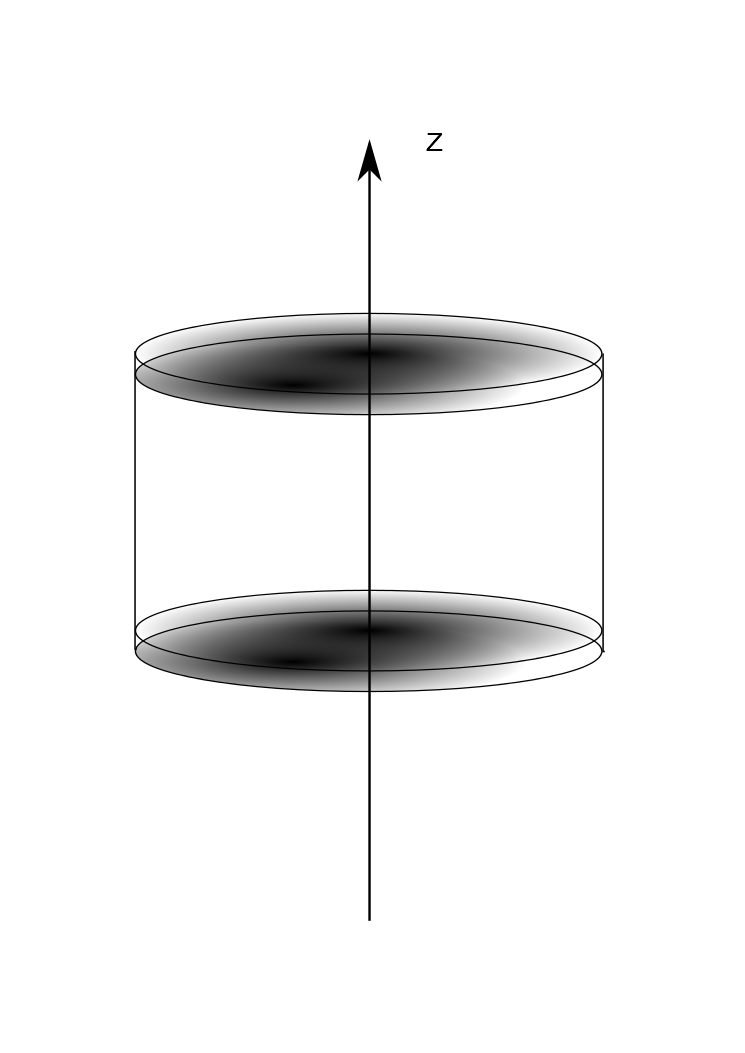
\includegraphics[width=60mm]{Figure3.png}
\end{center}

The top of the cylinder is given by:

\begin{equation}
\int KdA=-\frac{1}{2}\int^{R}_{0}\int^{2\pi}_{0}\frac{d}{dr}\left(\frac{1}{\sqrt{EG}}\frac{dG}{dr}\right)drd\phi
\end{equation}

And:

\begin{equation}
\left(\frac{1}{\sqrt{EG}}\frac{dG}{dr}\right)=2e^{-\nu}\left(1-r\partial_{r}\lambda\right)
\end{equation}

Then:

\begin{equation}
\int KdA=2\pi[e^{-\nu}\left(r\partial_{r}\lambda-1\right)]^{R}_{0}
\end{equation}

Taking the limit as $R\rightarrow\infty$ and recalling elementary flatness (Equation (\ref{eq:elem-flat}), the Gauss-Bonnet theorem gives:

\begin{equation}
K=2\pi\left(1-e^{-\nu (r,z)}\right)\delta(r)
\end{equation}

Where the delta-function $\delta(r)$ is given by \cite{araujo_static_1995}:

\begin{equation}
\delta(r)=\int^{\infty}_{0} \int^{2\pi}_{0} \delta (r)e^{2\left(\lambda-\nu\right)}rdrd\phi =1
\end{equation} 

The two-dimensional sub-manifold in $\left(r,\phi\right)$ is diagonal, so that the only non vanishing components of the Ricci tensor are $R_{rr}=R_{\phi\phi}=K$. Applying Einstein's equation (Equation (\ref{eq:einstein})) we have:

\begin{equation}
T_{zz}=\frac{1}{8\pi G}2\pi\left(1-e^{-\nu (r,z)}\right)\delta(r)
\end{equation} 

Thus:

\begin{equation}
F=\int T_{zz}dA=\frac{1}{4G}\left(1-e^{-\nu (r,z)}\right)
\end{equation}

Where G is Newton's constant. Looking over our Newtonian potentials ($\lambda$) from Equation (\ref{eq:2-m}) (which suppressed factors of G) and expanding the exponential:

\begin{equation}
e^{-\nu\left(0,z\right)}=1+\left(-\nu\left(0,z\right)\right)+\left(-\nu\left(0,z\right)\right)^{2}+...
\end{equation}

After applying the solution for $\nu(0,z)$ from Equation (\ref{eq:nu_r=0}), the first order approximation is (recalling that $\mu_{1}=Gm_{1}$ and $\mu_{2}=Gm_{2}$):

\begin{equation}
F=\frac{Gm_{1}m_{2}}{\left(z_{1}-z_{2}\right)^{2}}
\end{equation}

Where higher order terms of $\nu\left(0,z\right)$ are corrections to Newton's law.

\section{Application to Causal Dynamical Triangulations}

Causal Dynamical Triangulations uses a path integral over all possible
configurations between boundary conditions. The path integral is given
by:

\begin{equation}
  \label{eq:path-integral}
Z=\int \mathcal{D}[g]e^{iS_ {EH}}
\end{equation}

Where:

\begin{equation}
  \label{eq:einstein-hilbert-action}
  S_{EH}=\frac{1}{16\pi G}\int_{M}d^4 x\sqrt{-g}\left(R-2\Lambda\right)
\end{equation}

Given \eqref{eq:path-integral} and \cite{kommu2011} 

\subsection{Regge Calculus}



\bibliographystyle{ieeetr}
\bibliography{cdt-newtonian-limit-biblio}


\end{document}

% LocalWords:  xport
